\section{Class 17}

\subsection{Multiple lienar regression}

\subsubsection{Setup}

Under MLR, assume the outcome variable $y_i$ is linearly related to $p$ covariates, with $n$ samples, we have 
\[
    y_i  = \beta_0 + \beta_1 x_{1i} + \hdots + \beta_p x_{pi} + \epsilon_i
\]

Where the error variables are assumed 
\[
    \epsilon_i \sim N(0, \sigma^2)
\]
i.e. error terms are assumed to have mean 0, and are independently and normally distributed with identical variances. 

In matrix form, we write 
\begin{align*}
    \bm{Y} &= \bm{X \beta} + \bm{\epsilon}\\ 
    \begin{pmatrix} y_1 \\ y_2 \\ \vdots \\ y_n \end{pmatrix} &= 
    \begin{pmatrix} 
      1 & x_{11}  & \hdots & x_{p1} \\
      2 & x_{12}  & \hdots & x_{p2} \\
      \vdots & \vdots & \vdots & \vdots \\
      n & x_{1n}  & \hdots & x_{pn}
    \end{pmatrix} 
    \begin{pmatrix} 
      \beta_0 \\ \beta_1 \\ \vdots \\ \beta_p  
    \end{pmatrix} + 
    \begin{pmatrix} 
      \epsilon_0 \\ \epsilon_1 \\ \vdots \\ \epsilon_p  
    \end{pmatrix}
\end{align*}
i.e. 
\begin{itemize}
    \item $\bm{Y} \in \mathbb{R}^{n \times 1}$
    \item $\bm{X} \in \mathbb{R}^{n \times (p + 1)}$
    \item $\bm{\beta} \in \mathbb{R}^{p \times 1}$
    \item $\bm{\epsilon} \in \mathbb{R}^{n \times 1}$
\end{itemize} 

\subsubsection{Least Square Estimate}
\begin{definition}
    (Least square estimate of MLR): Suppose 
    \[
    \bm{Y} = \bm{X \beta} + \bm{\epsilon}, \bm{\epsilon} \sim N_p \left( \bm{0}, \sigma^2 \bm{I} \right) 
    \]
    The least square estimate of $\beta$, denoted $\hat{\beta}$ is defined as 
    \begin{align*}
        \hat{\bm{\beta}} &= \arg \min_{\bm{\beta}} \lVert \bm{Y} - \bm{X \beta} \rVert_2^2 \\
        &= \arg \min_{ \bm{\beta}} \sum\limits_{i = 1}^{n}  \left( y_i - \bm{x}_i^{\top} \bm{\beta} \right)^2
    \end{align*}
    Where 
    \[
        \bm{x}_i = \begin{pmatrix} 
          1 \\ x_{1i}   \\ x_{2i} \\ \vdots \\ x_{pi}
        \end{pmatrix}
    \]
\end{definition}

\begin{result}
    If $\rank(\bm{X}) = p + 1$, then the closed form solution for $ \hat{ \bm{\beta}}$ is 
    \[
        \hat{ \bm{\beta}} = \left( \bm{X}^{\top} \bm{X} \right)^{-1} \bm{X}^{\top} \bm{Y}
    \]
\end{result}

\begin{proof}
    We can express the sum of squared errors as 
    \begin{align*}
        \lVert \bm{Y} - \bm{X \beta} \rVert_2^2 &= \left( \bm{Y} - \bm{X \beta} \right)^{\top} \left( \bm{Y} - \bm{X \beta} \right)  \\
        &= \bm{Y}^{\top} \bm{Y} - 2 \bm{\beta}^{\top}\bm{X}^{\top}\bm{Y} + \bm{\beta}^{\top}\bm{X}^{\top}\bm{X}\bm{\beta}
    \end{align*}

    Taking the derivative with respect to $\bm{\beta}$ gives the gradient vector 
    \begin{align*}
        \nabla_{ \bm{\beta}} \lVert \bm{Y} - \bm{X \beta} \rVert^2 &= -2 \bm{X}^{\top} \bm{Y} + 2 \bm{X}^{\top} \bm{X} \bm{\beta}
    \end{align*}

    Setting this equal to $\bm{0}$, we get the \textbf{normal equation} 
    \[
        \bm{X}^{\top} \bm{X \beta} = \bm{X}^{\top} \bm{XY}
    \]

    Since $\bm{X}$ has full column rank (i.e. rank $p + 1$), $\rank(\bm{X}^{\top}\bm{X}) = p + 1$, hence 
    \begin{align*}
        \hat{ \bm{ \beta}} = \left( \bm{X}^{\top} \bm{X} \right)^{-1} \bm{X}^{\top}\bm{Y}
    \end{align*}
\end{proof}

\subsubsection{Properties of the LS estimate} 

\begin{result}
    \textbf{The LS esimate is unbiased}
    \begin{align*}
        \mathbb{E}\left[ \hat{ \bm{ \beta}}\right]  &= \left( \bm{X}^{\top} \bm{X} \right)^{-1} \bm{X}^{\top}\mathbb{E}\left[ \bm{Y}\right]  \\
        &= \left( \bm{X}^{\top} \bm{X} \right)^{-1} \bm{X}^{\top} \bm{X \beta}  \\ 
        &= \bm{\beta}
    \end{align*}
\end{result}

\begin{result}
    \textbf{Variance of}  $\hat{\bm{\beta}}$ 
    \begin{align*}
        Var( \hat{ \bm{\beta}}) &= Var \left( \bm{AY} \right)  \\
        &= \bm{A} Var( \bm{Y}) \bm{A}^{\top} \\
        &= \left(\bm{X}^{\top} \bm{X}\right)^{\top} \bm{X}^{\top} \sigma^2 \bm{IX} \left( \bm{X}^{\top} \bm{X} \right)^{-1} \\
        &= \sigma^2 \left( \bm{X}^{\top} \bm{X} \right)^{-1}
    \end{align*}
\end{result}

\begin{result}
    \textbf{The LS estimate is normally distributed}. \\

    We know that 
    \[
        \bm{Y} \sim N_n \left( \bm{X \beta}, \sigma^2 I \right) 
    \]
    Hence $ \hat{ \bm{ \beta}} = \bm{AY}, \bm{A} = (\bm{X}^{\top} \bm{X})^{-1} \bm{X}^{\top}$ is a linear combination of normals, hence 
    \begin{align*}
        \hat{ \bm{\beta}} \sim N_{p + 1} \left( \bm{\beta}, \sigma^2 \left( \bm{X}^{\top} \bm{X} \right)^{-1}  \right) 
    \end{align*}
\end{result}

\subsubsection{Geometric interpretations of LS estimates}

\begin{center}
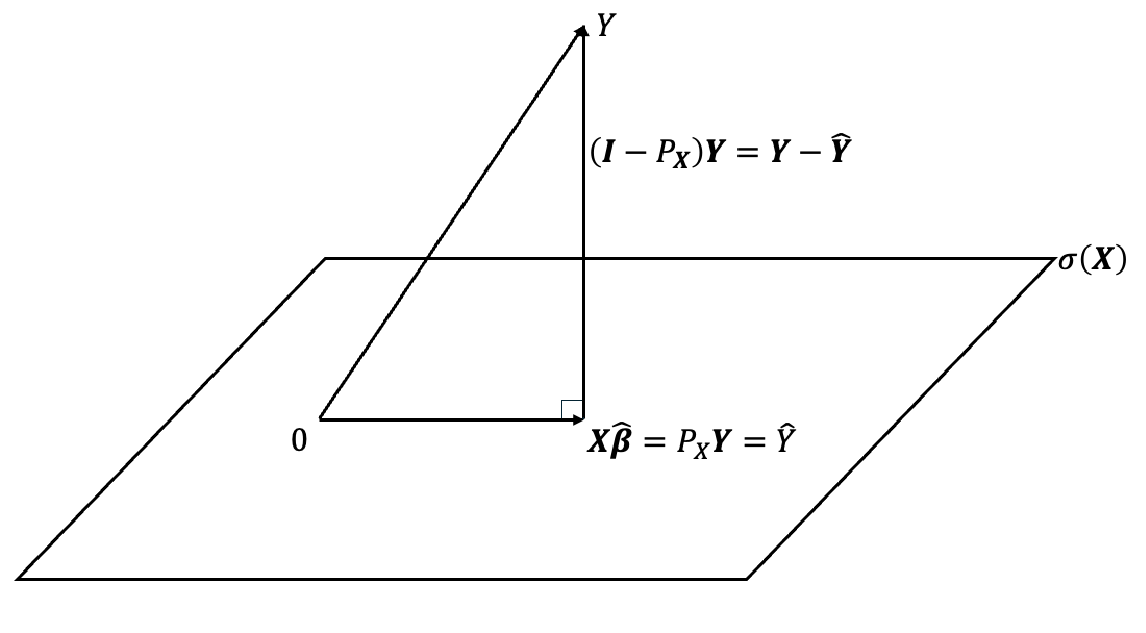
\includegraphics[width = 0.5\textwidth]{figures/fig_17_1.pdf}
\end{center}

\begin{remark}
    Any vector $\bm{v} = \bm{X \beta}$ is a linear combination of the columns of $\bm{X}$. Let $\sigma(\bm{X})$ denote the column space of $\bm{X}$. \\

    The LS estimate is obtained by finding $\bm{X \hat{\beta}} \in \sigma( \bm{X})$  that is the closest Euclidean distance to $\bm{Y} \in \mathbb{R}^n$. 

    The predicted value is 
    \begin{align*}
        \hat{ \bm{Y}} &= \bm{X \hat{ \beta}} \\
        &= \bm{X} \left( \bm{X}^{\top} \bm{X} \right)^{-1} \bm{X}^{\top} \bm{Y} \\
        &= \bm{P_X} \bm{Y}
    \end{align*}
\end{remark}

\begin{result}
    \textbf{Properties of the projection matrix} $\bm{P_X}$ 
    \begin{enumerate}
        \item For any $\bm{v} \in \mathbb{R}^n$, $\bm{P_X v} \in \sigma( \bm{X})$ 
        \item If $\bm{v} \in \sigma( \bm{X}), \bm{P_X v} = \bm{v}$ 
        \item $\bm{P_X}$ is idempotent, 
        \begin{align*}
            \bm{P_X^2} &= \bm{X} \left( \bm{X}^{\top} \bm{x} \right)^{-1} \bm{X}^{\top}\bm{X} \left(  \bm{X}^{\top}\bm{X} \right)^{-1} \bm{X}^{\top} \\
            &= \bm{P_X}
        \end{align*}
    \end{enumerate}
\end{result}

\begin{definition}
    (Residuals): Define the residuals as 
    \begin{align*}
        \bm{E} &= \begin{pmatrix}  
          E_1 \\ E_2 \\ \hdots \\ E_n  
        \end{pmatrix}  \\
        &= \bm{Y}- \hat{\bm{Y}}  \\
        &= \bm{Y} - \bm{X \hat{\beta}} \\
        &= (\bm{I} - \bm{P_X}) \bm{Y}
    \end{align*}
\end{definition}

\begin{result}
    The predicted value $\hat{ \bm{Y}}$ is orthogonal to the residual $\bm{E}$.

    \begin{align*}
        \bm{E}^{\top} \hat{\bm{Y}} &= \bm{Y}^{\top} \left( \bm{I} - \bm{P_X} \right) \bm{P_X} \bm{Y} \\
        &= \bm{0}
    \end{align*}

    Hence by Pythagoras theorem 
    \begin{align*}
        \lVert \bm{Y} \rVert^2 &= \lVert \hat{\bm{Y}} \rVert^2 + \lVert \bm{E} \rVert^2 \\
        &= \lVert \bm{P_X Y} \rVert^2 + \lVert \left( \bm{I} - \bm{P_X} \right) \bm{Y}  \rVert^2
    \end{align*}
\end{result}



\newpage